\chapter{Monte-Carlo Simulations of the SPM} 
\label{sec:numerics}
We now have numerical results for SPM systems using TRM analysis; however, this only allows us to study
relatively small systems. In order to study larger ones, we have used Monte-Carlo methods. In this
chapter, we will discuss the methods we used, the results they yielded and their meaning, with 
particular emphasis on what they tell us about the suspected transition between low and high-$\lambda$
behaviours.
\section{Numerical Simulations of Continuous-Time Markov Processes}
Here we will discuss the theory behind the Monte-Carlo methods used to simulated continuous-time Markov
processes. We will assume throughout that we have the computational means to produce pseudorandom
floating-point numbers in a way which which closely approximates the uniform real distribution over $(0, 1)$.
\subsection{Purpose of Monte-Carlo Methods}
We should first really describe what we mean by a Monte-Carlo method. In essence, Monte-Carlo methods
refer to numerical routines in which we attempt to characterise an unknown distribution, generated 
via known rules, by using
pseudorandom numbers in order to produce sample data which is hopefully faithful to the original 
distribution, at least in terms of the statistics we are trying to calculate. A good example of a
commonly-used Monte-Carlo method in Physics is the Metropolis-Hastings algorithm, which in its original
for is used to calculate statistics for equilibrium statistical mechanics systems.

In our situation, we wish to be able to mimic a continuous-time discrete-state Markov process.
As we saw in Chap.~\ref{sec:TRM}, the state space for a TRM system of size $L$ scales as
$\mathcal{O}(2^L$); thus we quickly run out of size if we try to consider exactly probability distributions, which correspond to
vectors in $\mathbb{R}^{L^2}$. We can, however, store individual configurations, which only occupy
$\mathcal{O}(L)$ space. Therefore, we need to find a way to produce trajectories through the discrete
state space which sample the actual space of system trajectories well enough to allow us to access the
statistics we want. Of course, there isn't a unique ``best'' way to do this. We have considered two
contrasting methods, which differ primarily in the way in which they convert the original continuous 
time into discrete steps which we can use in an algorithm.

\subsection{Evenly-Spaced Timesteps}

If we wished to numerically approximate an ODE system, one might use the Euler forward or 
Runge-Kutte methods. These both involve discretising time simply by dividing it into evenly-sized
pieces, and then converting the ODE into a discrete form by using finite differences to
approximate derivatives. We need to be careful to choose a small enough timestep for
the approximation to the derivative to remain good, but otherwise it is a very simple and 
effective approach.

We can do a very similar technique with continuous time Markov processes. In our SPM system,
if we ignore the boundaries, there are two rates, $1$ and $\lambda$, and our system is 
homogeneous. Let us represent the system with a binary array of length $L+2$, with $L$ sites for the bulk
and a site each representing the boundaries. Therefore, in order to simulate the action of the SPM as
defined in <reference to appropriate section in
introduction>, we can use the following recipe:
\begin{enumerate}
 \item \textbf{START}. Advance time by $\Delta t$. Pick a site, which we will call
 Site,
 (of which there are $L+2$) at random. If the site chosen is one of the boundaries with density $\rho$,
 reset the site to be occupied with probability $\rho$ and unoccupied with probability $1-\rho$.
 \item If Site is occupied, pick one of the two adjacent sites, which we will call Target, at random with equal probability.
 This will be the site we attempt to move into. If it is not, go back to \textbf{START}.
 \item \textit{If Site is not on the boundary}: If Target is occupied, go to \textbf{START}. Otherwise, consider the other adjacent site,
 which we will refer to as Rear. If Rear is empty, move the particle in Site into Target 
 randomly with
 probability $\frac{1}{1+\lambda}$; otherwise, move the particle with probability
 $\frac{\lambda}{1+\lambda}$. Return to \textbf{START}. 
 \newline \textit{If Site is on the boundary}: If Target is outside the system, go to \textbf{START}.
 If Target is occupied, go to \textbf{START}. Assign an occupation value for Rear randomly, occupied
 with probability $\rho$, unoccupied with probability $1-\rho$, where $\rho$ is the density of the relevant
 boundary. Now, if Rear is empty, move the particle in Site into Target 
 randomly with  probability $\frac{1}{1+\lambda}$; otherwise, move the particle with probability
 $\frac{\lambda}{1+\lambda}$. Return to \textbf{START}.
\end{enumerate}
We define $\Delta t$ via 
\begin{equation}
 \Delta t = \frac{\tau_0}{L (1+\lambda)}.
\end{equation}
In terms of the algorithm's correctness at producing reasonable trajectories, we simply need note that
the rates at which particular transitions should occur are in the correct proportions, and that the boundaries result in the correct densities in equilibrium;
then, we just need
to verify that the rate at which free particles move is the correct one in absolute terms, which it is,
and we're done. 

For Monte-Carlo methods, we generally rate their performance by the amount of computational
power required to explore a given amount of the probability space. In methods in which we
are exploring this space by advancing though time (and invoking ergodicity) we desire methods
which move us quickly through time whilst maintaining good sampling and performing little computation.

The advantage of this method is that it is very simple; thus, there aren't too many opportunities
for error when writing the code, it uses very little memory (all calculations can be performed
in-place), and each iteration should be very fast as there are very few overheads. It should also
produce trajectories which are good samples of the original probability distribution we are 
trying to replicate.


If $\lambda$
is close to $1$, the probability of rejection (i.e. a step which results in no overall change to
the system) is $\sim\frac{1}{2}$, and this is the situation in which the algorithm really shines; similarly
it also performs well for large or small $lambda$ if the system density is very high or very low
respectively. For extreme $\lambda$ in general however, performance drops off considerably, as
we are often performing lots of calculations and advancing time very little, and thus not seeing
much of the distribution simply because we aren't moving much.

We could have made this code marginally more efficient by making the more likely moves certain, and
correspondingly adjusting the timestep size $\Delta t$ to account for this; however, this only
improves efficiency by a factor of around $2$ , whilst making the code more complicated, so as
we only used this method to verify the results of our main code we didn't bother.
It is possible for us to get
around this issue by advancing time in a variable fashion, although this comes at the cost of
a little more computation per iteration.

\subsection{The N-Fold Way, or Gillespie Algorithm}
A popular way to produce trajectories for a continuous-time Markov process is the N-Fold Way, also known as
BKL, or Gillespie Algorithm~\cite{Bortz1975, Prados1997, voterKMC}. It evolves us through time as follows:
\begin{enumerate}
 \item \textbf{START}: Make a list of all states which can be transitioned to in a single move from the 
 current state, and the associated rates at which this occurs.
 \item Weight each successor state by the transition rate into it, and then select a successor state by
 random selection from a uniform distribution over the weighted possible successors. Change the system
 state to the chosen successor, and retain the associated rate. \label{weightingChoose}
 \item Now advance time by an increment chosen from an exponential distribution whose decay rate 
 is the rate retained from the previous step. Go back to \textbf{START}. \label{timestepChoose}
\end{enumerate}
Now we just need to supply the rates <from introduction> that define the SPM, along with some additional rates describing processes at the boundary. Specifically, we use the method described 
in~\ref{sec:CTMPBoundaries} to do this, whereby we have a double layer of ``blinking'' boundary sites
and sites in the internal layer undergo the same transitions as in the bulk. However, unlike in our TRM
calculations, we should not set the incoming and outgoing rates to be extremely high, as then these rather
trivial processes come to dominate the calculation and waste our computing time. Instead, we set them to
be proportional to the geometric mean of $1$ and $\lambda$, and thus in the language of~\ref{eq:blinkRates}
this corresponds to setting $B_0 = \sqrt{\lambda}$. This way the boundaries refresh often, but not too
often, and should still act as suitable reservoirs.

We will get into the fine details about how the software we use implements KMC in Sec.~\ref{sec:kmcLib}.
Let us instead discuss how we obtain the required probability distributions using the uniform distribution
on $(0, 1)$, $U(0, 1)$:
\begin{itemize}
 \item We can randomly choose the successor state required in step~\ref{weightingChoose} by
 creating a list of weighted partial sums. If the transition rate from the current state the $i^\mathrm{th}$
 potential successor state is $k_i$, then let us define $k_\mathrm{Tot.} = \sum_{i}^n$, where $n$ is the
 number of potential successors. Create the list of partial sums via $s_i = \sum_j^i k_j$, then generate
 the random number $u = r k_\mathrm{Tot.}$ where $r$ is drawn from $U(0, 1)$. We can then use a binary
 search to find $i: s_{i-1} \le u \le s_i$, and then this $i$ indicates the successor state which has been
 chosen. This process is illustrated more visually in Fig.~\ref{fig:weightChoice}.
 \item In step~\ref{timestepChoose}, we need to generate random numbers in an exponential distribution
 with decay rate $k$. We can do this by generating $r$ from $U(0, 1)$, and then $w = -\frac{1}{k} \log{r}$
 follows the desired distribution.
\end{itemize}
\begin{figure}[h!]
 \caption[Illustration of the method for choosing successor states in the n-fold way.]{\label{fig:weightChoice} 
 An illustration of the suggested method for choosing a successor state in the n-fold way. Reproduced
 from~\cite{voterKMC}.
 }
  \begin{center}
 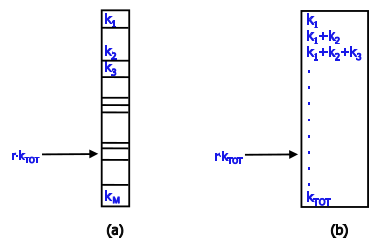
\includegraphics[width=1.0\textwidth]{numerics/images/nFoldWayRates}
  \end{center}
\end{figure}

With this method, we certainly advance time every step, so we are not ``wasting'' steps as when we use even 
timestepping; this comes at the cost of having to compute all possible transitions from the current state.
For our SPM, a given state has $\mathcal{O}(L)$ possible transitions.


\section{Implementation of Monte Carlo Methods}
\subsection{Our Implementation of a Metropolis-Hastings}
\subsection{\texttt{KMCLib}} \label{sec:kmcLib}
Talk about how it works, why I picked it over other implementations.
\subsection{Running our Monte-Carlo Calculations}
How calculations are managed day-to-day.

\section{1D Calculation Results}
\subsection{Calculational Choices}
\subsection{Flow Patterns}
\subsection{Current}
\subsection{Density}
\subsection{Diffusion Coefficient}

\section{2D Calculation Results}
\subsection{Calculational Choices}
\subsection{Results}

\section{Conclusions}
